\onehalfspacing
\section{Đề số 15}
\graphicspath{{./img/}}
\begin{bt} 
    \hfill
	\begin{enumerate}[a.]
		\item Thực hiện phép tính:
        $$
        \mathrm{A}=\frac{9 \cdot 6^9 \cdot 120-4^6 \cdot 9^6}{8^4 \cdot 3^{13}-6^{12}} ; \quad \mathrm{B}=\frac{10}{7 \cdot 12}+\frac{10}{12 \cdot 17}+\frac{10}{17 \cdot 22}+\ldots+\frac{10}{2012 \cdot 2017}+\frac{10}{2017 \cdot 2022}
        $$
        \item Cho a, b, c là ba số thực khác 0 , thoả mãn : $\frac{a+b-c}{c}=\frac{b+c-a}{a}=\frac{a+c-b}{b}$.
        Hãy tính giá trị của biểu thức $B=\left(1+\frac{b}{a}\right) \cdot\left(1+\frac{a}{c}\right) \cdot\left(1+\frac{c}{b}\right)$.
        \item Tính giá trị của đa thức $f(x)=x^5-2018 x^4+2016 x^3+2018 x^2-2016 x-2017$ tại $x=2017$
	\end{enumerate}
	\loigiai{
        \begin{enumerate}
            \item $A=\frac{9 \cdot 6^9 \cdot 120-4^6 \cdot 9^6}{8^4 \cdot 3^{12}-6^{12}}=\frac{3^2 \cdot 2^9 \cdot 3^9 \cdot 2^3 \cdot 3 \cdot 5-2^{12} \cdot 3^{12}}{2^{12} \cdot 3^{13}-2^{12} \cdot 3^{12}} \triangleleft \\[5pt]
            =\frac{3^{12} \cdot 2^{12} \cdot 5-2^{12} \cdot 3^{12}}{2^{12} \cdot 3^{12}(3-1)}=\frac{3^{12} \cdot 2^{12}(5-1)}{2^{12} \cdot 3^{12} \cdot 2} \\[5pt]
            =\frac{5-1}{2}=2 \\[5pt]
            \text { Vậy } A=2 \\[5pt]
            B=\frac{10}{7 \cdot 12}+\frac{10}{12 \cdot 17}+\frac{10}{17 \cdot 22}+\ldots+\frac{10}{2012 \cdot 2017}+\frac{10}{2017 \cdot 2022} \\[5pt]
            =2 \cdot\left(\frac{5}{7 \cdot 12}+\frac{5}{12 \cdot 17}+\frac{5}{17 \cdot 22}+\ldots .+\frac{5}{2012 \cdot 2017}+\frac{5}{2017 \cdot 2022}\right) \\[5pt]
            =2\left(\frac{1}{7}-\frac{1}{12}+\frac{1}{12}-\frac{1}{17}+\frac{1}{17}-\frac{1}{22}+\ldots .+\frac{1}{2012}-\frac{1}{2017}+\frac{1}{2017}-\frac{1}{2022}\right) \\[5pt]
            =2\left(\frac{1}{7}-\frac{1}{2022}\right)=2 \cdot \frac{2022-7}{2022 \cdot 7}=\frac{2015}{7077} \\[5pt]
            \text { Vậy } B=\frac{2015}{7077}$
            \item +) Nếu a $+b+c \neq 0$\\[5pt]
            Theo tính chất dãy tỉ số bằng nhau, ta có:\\[5pt]
            $\frac{a+b-c}{c}=\frac{b+c-a}{a}=\frac{c+a-b}{b}=\frac{a+b-c+b+c-a+c+a-b}{a+b+c}=1 \\[5pt]
            \text { mà } \frac{a+b-c}{c}+1=\frac{b+c-a}{a}+1=\frac{c+a-b}{b}+1=2 \\[5pt]
            \Rightarrow \frac{a+b}{c}=\frac{b+c}{a}=\frac{c+a}{b}=2 \\[5pt]
            \text { Vậy B }=\left(1+\frac{b}{a}\right)\left(1+\frac{a}{c}\right)\left(1+\frac{c}{b}\right)=\left(\frac{b+a}{a}\right)\left(\frac{c+a}{c}\right)\left(\frac{b+c}{b}\right)=8$\\[5pt]
            +) Nếu $a+b+c=0$\\[5pt]
            Theo tính chất dãy tỉ số bằng nhau, ta có:\\[5pt]
            $\frac{a+b-c}{c}=\frac{b+c-a}{a}=\frac{c+a-b}{b}=\frac{a+b-c+b+c-a+c+a-b}{a+b+c}=0\\[5pt]
            \text { mà } \frac{a+b-c}{c}+1=\frac{b+c-a}{a}+1=\frac{c+a-b}{b}+1=1 \\[5pt]
            \Rightarrow \frac{a+b}{c}=\frac{b+c}{a}=\frac{c+a}{b}=1 \\[5pt]
            \text { Vậy B }=\left(1+\frac{b}{a}\right)\left(1+\frac{a}{c}\right)\left(1+\frac{c}{b}\right)=\left(\frac{b+a}{a}\right)\left(\frac{c+a}{c}\right)\left(\frac{b+c}{b}\right)=1$
            \item Tính giá trị của đa thức:\\[5pt]
            $f(x)=x^5-2018 x^4+2016 x^3+2018 x^2-2016 x-2017$ tại $\mathrm{x}=2017$\\[5pt]
            Ta có $x=2017 \Rightarrow\left\{\begin{array}{l}2018=x+1 \\[5pt] 2016=x-1\end{array}\right.$.\\[5pt] 
            Khi đó ta có:\\[5pt]
            $f(2017) =x^5-(x+1) x^4+(x-1) x^3+(x+1) x^2-(x-1) x-x \\[5pt]
            =x^5-x^5-x^4+x^4-x^3+x^3+x^2-x^2+x-x
            = 0$\\[5pt]
            Vậy $f(2017)=0$
        \end{enumerate}
    } 
\end{bt}

\begin{bt}
    \hfill
    \begin{enumerate}
        \item Cho $\frac{3 x-2 y}{4}=\frac{2 z-4 x}{3}=\frac{4 y-3 z}{2}$. Chứng minh rằng : $\frac{x}{2}=\frac{y}{3}=\frac{z}{4}$.
        \item Tìm $x, y, z$ biết: $\quad\left|x-\frac{1}{2}\right|+\left|y+\frac{2}{3}\right|+\left|x^2+x z\right|=0$
    \end{enumerate}
    \loigiai{
    \begin{enumerate}
        \item Theo bài ra ta có: $\frac{3 x-2 y}{4}=\frac{2 z-4 x}{3}=\frac{4 y-3 z}{2}$\\[5pt]
        Áp dụng tính chất của dãy tỉ số bằng nhau ta có:\\[5pt]
        $\Rightarrow \frac{12 x-8 y}{16}=\frac{6 z-12 x}{9}=\frac{8 y-6 z}{4}=\frac{12 x-8 y+6 z-12 x+8 y-6 z}{16+9+4}=0 \\[5pt]
        \Rightarrow\left\{\begin{array} { l } 
        { 1 2 x - 8 y = 0 } \\
        { 8 y - 6 z = 0 }
        \end{array} \Rightarrow \left\{\begin{array}{l}
        12 x=8 y \\
        8 y=6 z
        \end{array} \Rightarrow 12 x=8 y=6 z\right.\right.\\[5pt]
        \Rightarrow \frac{12 x}{24}=\frac{8 y}{24}=\frac{6 z}{24}\\[8pt] \Leftrightarrow \frac{x}{2}=\frac{y}{3}=\frac{z}{4}(\mathrm{dpcm})$
        \item Áp dụng tính chất $|A| \geq 0$\\[5pt]
        $
        \Rightarrow\left\{\begin{array} { l } 
        { | x - \frac { 1 } { 2 } | = 0 } \\
        { | y + \frac { 2 } { 3 } | = 0 } \\
        { | x ^ { 2 } + x z | = 0 }
        \end{array} \Rightarrow \left\{\begin{array} { l } 
        { x - \frac { 1 } { 2 } = 0 } \\
        { y + \frac { 2 } { 3 } = 0 } \\
        { x ( x + z ) = 0 }
        \end{array} \Rightarrow \left\{\begin{array}{l}
        x=\frac{1}{2} \\
        y=-\frac{2}{3} \\
        z=-x=-\frac{1}{2}
        \end{array}\right.\right.\right.
        $\\[5pt]
        Vậy $\mathrm{x}=\frac{1}{2} ; \mathrm{y}=-\frac{2}{3} ; \mathrm{z}=-\frac{1}{2}$
    \end{enumerate}
        }
\end{bt}

\begin{bt}
	\hfill
	\begin{enumerate}[a.]
		\item Tìm các cặp số tự nhiên $(\mathrm{x} ; \mathrm{y})$ sao cho: $49-\mathrm{y}^2=12(\mathrm{x}-2001)^2$
        \item Cho $\left|2019 x_1-2018 y_1\right|+\left|2019 x_2-2018 y_2\right|+\ldots+\left|2019 x_{2018}-2018 y_{2018}\right| \leq 0$. Chứng minh
        $$
        \frac{x_1+x_2+x_3+\ldots+x_{2018}}{y_1+y_2+y_3+\ldots+y_{2018}}=\frac{2018}{2019} \text {. }
        $$
        \item Một cửa hàng có ba cuộn vải, tổng chiều dài ba cuộn vải đó là $186 \mathrm{~m}$, giá tiền mỗi mét vải của ba cuộn là như nhau. Sau khi bán được một ngày cửa hàng còn lại $\frac{2}{3}$ cuộn thứ nhất, $\frac{1}{3}$ cuộn thứ hai, $\frac{3}{5}$ cuộn thứ ba. Số tiền bán được của ba cuộn thứ nhất, thứ hai, thứ ba lần lượt tỉ lệ với $2 ; 3 ; 2$. Tính xem trong ngày đó cửa hàng đã bán được bao nhiêu mét vải mỗi cuộn.
	\end{enumerate}
	\loigiai{
        \begin{enumerate}
            \item Xét đẳng thức: $49-y^2=12(x-2001)^2$.\\[5pt]
            Vế phải là mộ số chẵn không âm nên y là một số lẻ và không lớn hơn 7.\\[5pt]
            Khi $\mathrm{y}=1 \Rightarrow \mathrm{x}=2003$ và $\mathrm{x}=1999$\\[5pt]
            Khi $y=3$ không có giá trị $x \in N$\\[5pt]
            Khi $y=5$ không có giá trị $x \in \mathrm{N}$\\[5pt]
            Khi $\mathrm{y}=7 \Rightarrow \mathrm{x}=2011$\\[5pt]
            Vậy các cặp (x; y) cần tìm là $(2003 ; 1) ;(1999 ; 1)$; (2001; 7)
            \item Ta có:\\[5pt]
            $\left|2019 x_1-2018 y_1\right| \geq 0 \\[5pt]
            \left|2019 x_2-2018 y_2\right| \geq 0 \\[5pt]
            \ldots \\[5pt]
            \left|2019 x_{2018}-2018 y_{2018}\right| \geq 0 \\[5pt]
            \Rightarrow\left(2017 x_1-2016 y_1\right)^2+\left(2017 x_2-2016 y_2\right)^2+\ldots+\left(2017 x_{2016}-2016 y_{2016}\right)^2 \geq 0$\\[5pt]
            Theo bài ra ta có:\\[5pt]
            $\left|2019 x_1-2018 y_1\right|+\left|2019 x_2-2018 y_2\right|+\ldots+\left|2019 x_{2018}-2018 y_{2018}\right| \leq 0$\\[5pt]
            Suy ra:\\[5pt]
            $\left\{\begin{array}{c}
            \left|2019 x_1-2018 y_1\right|=0 \\
            \left|2019 x_2-2018 y_2\right|=0 \\
            \vdots \\
            \left|2019 x_{2018}-2018 y_{2018}\right|=0
            \end{array}\right. \\
            \Rightarrow\left\{\begin{array}{c}
            2019 x_1=2018 y_1 \\
            2019 x_2=2018 y_2 \\
            \vdots \\
            2019 x_{2018}=2018 y_{18}
            \end{array}\\[5pt] \Rightarrow \frac{x_1}{y_1}=\frac{x_2}{y_2}=\ldots=\frac{x_{2018}}{y_{2018}}=\frac{2018}{2019}\right. \\[5pt]$
            Áp dụng tính chất của dãy tỉ số bằng nhau ta được:\\[5pt]
            $\frac{x_1}{y_1}=\frac{x_2}{y_2}=\ldots=\frac{x_{2018}}{y_{2018}}=\frac{x_1+x_2+\ldots+x_{2018}}{y_1+y_2+\ldots+y_{2018}} \\[5pt]
            \text {Từ (1) và (2) suy ra } \frac{x_1+x_2+x_3+\ldots+x_{2018}}{y_1+y_2+y_3+\ldots+y_{2018}}=\frac{2018}{2019}$(đpcm)
            \item Gọi chiều dài cuộn vải thứ nhât, thứ hai, thứ ba lần lượt là $x, y, z(m)$ ĐK: $0<x, y, z<186$\\[5pt]
            +) Tổng chiều dài ba cuộn vải đó là $186 \mathrm{~m} \Rightarrow \mathrm{x}+\mathrm{y}+\mathrm{z}=186$\\[5pt]
            +) Sau khi bán được một ngày cửa hàng còn lại $\frac{2}{3}$ cuộn thứ nhất, $\frac{1}{3}$ cuộn thứ hai, $\frac{3}{5}$ cuộn thứ ba\\[5pt]
            Trong ngày đó cửa hàng đã bán được số mét vải ở cuộn thứ nhất, thứ hai, thứ ba lần lượt là $\frac{x}{3}, \frac{2 y}{3}, \frac{2 z}{5}$ (mét)\\[5pt]
            +) Số tiền bán được của ba cuộn thứ nhất, thứ hai, thứ ba lần lượt tỉ lệ với 2; $3 ; 2$ và giá tiền mỗi mét vải của ba cuộn như nhau.\\[5pt]
            $\Rightarrow$ Số mét vải bán được của ba cuộn thứ nhất, thứ hai, thứ ba lần lượt tỉ lệ với 2; 3; 2\\[5pt]
            $\Rightarrow \frac{x}{3}: \frac{2 y}{3}: \frac{2 z}{5}=2: 3: 2 \Rightarrow \frac{2 x}{12}=\frac{2 y}{9}=\frac{2 z}{10}$\\[5pt]
            Áp dụng tính chất của dãy tỉ số bằng nhau ta được:\\[5pt] $\frac{x}{12}=\frac{y}{9}=\frac{z}{10}=\frac{x+y+z}{12+9+10}=\frac{186}{31}=6$\\[5pt]
            $\Rightarrow\left\{\begin{array}{l}
            x=72 \\
            y=54 \\
            z=60
            \end{array}\right. \text { (Thỏa mãn điều kiện) }$\\[5pt]
            Vậy trong ngày đó cửa hàng đã bán số mét vải ở cuộn thứ nhất, thứ hai, thứ ba lần lượt là : 24; 36; 24 (mét).
        \end{enumerate}
    } 
\end{bt}

\begin{bt}
	Cho tam giác $A B C, M$ là trung điểm của $B C$. Trên tia đối của của tia MA lấy điểm $\mathrm{E}$ sao cho $\mathrm{ME}=\mathrm{MA}$. Chứng minh rằng:
	\begin{enumerate}[a.]
		\item $\mathrm{AC}=\mathrm{EB}$ và $\mathrm{AC} / / \mathrm{BE}$
        \item Gọi I là một điểm trên $\mathrm{AC} ; \mathrm{K}$ là một điểm trên $\mathrm{EB}$ sao cho $\mathrm{AI}=\mathrm{EK}$. Chứng minh ba điểm I, M $\mathrm{K}$ thẳng hàng
        \item Từ E kẻ $E H \perp B C(H \in B C)$. Biết $H B E=50^{\circ} ; M E B=25^{\circ}$. Tính $H E M$ và $B M E$
    \end{enumerate}
	\loigiai{
        $$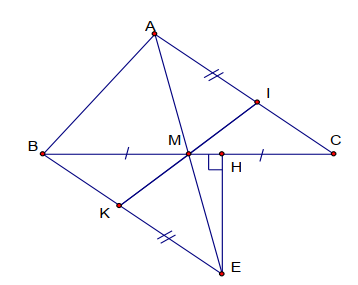
\includegraphics[width=0.5\textwidth]{15-4-lg.png}$$
        \begin{enumerate}
            \item Xét $\triangle A M C$ và $\triangle E M B$ có :
            $\mathrm{AM}=\mathrm{EM} \quad(\mathrm{gt}) \\[5pt]
            A M C=E M B \quad \text { (đối đỉnh }) \\[5pt]
            \mathrm{BM}=\mathrm{MC} \quad(\mathrm{gt}) \\[5pt]
            \text { Nên : } \triangle A M C=\Delta E M B \text { (c.g.c }) \\[5pt]
            \Rightarrow \mathrm{AC}=\mathrm{EB} \\[5pt]
            \text { Vì } \triangle A M C=\triangle E M B \\[5pt]\Rightarrow M A C=M E B$\\[5pt]
            Mà $M A C$ và $M E B$ là 2 góc có vị trí so le trong \\[5pt]Suy ra $\mathrm{AC} / / \mathrm{BE}$.
            \item Xét $\triangle A M I$ và $\triangle E M K$ có:\\[5pt]
            $\mathrm{AM}=\mathrm{EM}(\mathrm{gt}) \\[5pt]
            M A I=M E K \text { (vì } \triangle A M C=\triangle E M B) \\[5pt]
            \mathrm{AI}=\mathrm{EK} \text { (gt }) \\[5pt]
            \text { Nên } \triangle A M I=\Delta E M K(\text { c.g.c ) } \\[5pt]
            \text { Suy ra } A M I=E M K \\[5pt]
            \text { Mà } A M I+I M E=180^{\circ} \text { ( tính chất hai góc kề bù ) } \\[5pt]
            \Rightarrow \mathrm{EMK}+I M E=180^{\circ} \\[5pt]
            \Rightarrow \text { Ba điểm } \mathrm{I} ; \mathrm{M} ; \mathrm{K} \text { thẳng hàng }(\text { đpcm })$
            \item Trong tam giác vuông BHE ($H=90^{\circ}$) có $H B E=50^{\circ}$\\[5pt]
            $\Rightarrow H B E=90^{\circ}-H B E=90^{\circ}-50^{\circ}=40^{\circ} \\[5pt]
            \Rightarrow H E M=H E B-M E B=40^{\circ}-25^{\circ}=15^{\circ}$\\[5pt]
            $B M E$ là góc ngoài tại đỉnh $\mathrm{M}$ của $\triangle H E M$\\[5pt]
            Nên $B M E=H E M+M H E=15^{\circ}+90^{\circ}=105^{\circ}$
            ( định lý góc ngoài của tam giác)
        \end{enumerate}
    }
\end{bt}

\begin{bt}
    Tìm các số tự nhiên $x, y, z \neq 0$ thoả mãn điều kiện: $x+y+z=x y z$
\loigiai{
    Không mất tính tổng quát của bài toán giả sử $\mathrm{x} \leq \mathrm{y} \leq \mathrm{z}$\\[5pt]
    Vì $\mathrm{x}, \mathrm{y}$, $\mathrm{z}$ là các số tự nhiên khác $0 \Rightarrow 1 \leq \mathrm{x} \leq \mathrm{y} \leq \mathrm{z}$\\[5pt] 
    Ta có $\mathrm{x}+\mathrm{y}+\mathrm{z}=\mathrm{xyz} \quad(*)$\\[5pt]
    $\Rightarrow \frac{1}{y z}+\frac{1}{x z}+\frac{1}{x y}=1 \\[5pt]
    \Rightarrow 1 \leq \frac{1}{x^2}+\frac{1}{x^2}+\frac{1}{x^2}=\frac{3}{x^2} \\[8pt]
    \Rightarrow x^2 \leq 3 \Rightarrow x=1$\\[5pt]
    Thay vào $\left({ }^*\right)$ ta được:\\[5pt]
    $1+\mathrm{y}+\mathrm{z}=\mathrm{yz} \\[5pt]
    \Rightarrow (\mathrm{y}-1)(\mathrm{z}-1)=2 \\[5pt]
    \Rightarrow \left\{\begin{array} { l } 
    { \mathrm { y } - 1 = 1 } \\
    { \mathrm { z } - 1 = 2 }
    \end{array} \Rightarrow \left\{\begin{array}{l}
    \mathrm{y}=2 \\
    \mathrm{z}=3
    \end{array}\right.\right. \\[5pt]
    \Rightarrow (\mathrm{x}, \mathrm{y}, \mathrm{z})=(1 ; 2 ; 3)$\\[5pt]
    Vì vai trò của $\mathrm{x}, \mathrm{y}, \mathrm{z}$ như nhau nên các bộ số $(x, y, z)$ thoả mãn bài toán là :
    $$(1 ; 2 ; 3) ;(1 ; 3 ; 2) ;(2 ; 1 ; 3) ;(2 ; 3 ; 1) ;(3 ; 1 ; 2) ;(3 ; 2 ; 1)$$
}
\end{bt}

